\seite{}{DAEs und Bindungen}\anchorpage{1}{neu4}{4 · Differential-algebraische Gleichungen und Zwangsbedingungen}\ey{KAPITEL 4}\ptitle{Differential-algebraische Gleichungen und Zwangsbedingungen}
Ein Pendelgewicht darf einen Kreis entlanglaufen. Sein Ort kann die richtige Länge haben, obwohl seine Geschwindigkeit quer aus dem Kreis zeigt. Ein Schaltkreis kennt dieselbe Schwierigkeit in anderer Gestalt. Zwei gewählte Anfangsspannungen können die Maschenregel verletzen. Welche Daten dürfen wir frei vorgeben, und wie hält ein Integrator sie während der Bewegung miteinander verträglich?
\subt{Der Weg durch das Kapitel}
{\tblstart\begin{tabularx}{\linewidth}{@{}Yr@{}}\toprule
\hyperlink{abs4-1}{4.1 · Vom physikalischen Zwang zur Gleichung} & \pagelink{abs4-1}\\[2pt]
\hyperlink{abs4-2}{4.2 · Index und konsistente Bewegung} & \pagelink{abs4-2}\\[2pt]
\hyperlink{abs4-3}{4.3 · Indexreduktion, Drift und Projektion} & \pagelink{abs4-3}\\[2pt]
\hyperlink{abs4-4}{4.4 · Direkte DAE-Integration} & \pagelink{abs4-4}\\[2pt]
\bottomrule\end{tabularx}\par}
\par\vfill{\centering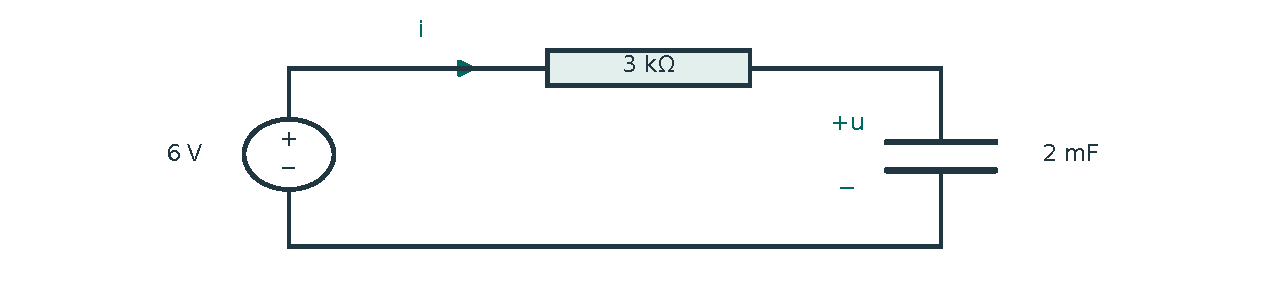
\includegraphics[width=.88\linewidth,height=49mm,keepaspectratio]{masche.pdf}\par}\capline{Die Maschengleichung hält die elektrischen Größen am selben Zeitpunkt zusammen.}
\seite{}{DAEs und Bindungen}\anchorpage{2}{abs4-1}{4.1 · Vom physikalischen Zwang zur Gleichung}\ey{ABSCHNITT 4.1}\ptitle{Vom physikalischen Zwang zur Gleichung}
\hypertarget{punkt4-1-1}{}\subt{4.1.1\enspace Mehrkörpermechanik und Kirchhoffsche Netze}
Der Faden zieht in radialer Richtung. Seine Spannung ist eine unbekannte Reaktion, die die vorgeschriebene Länge durchsetzt. Im elektrischen Knoten erzwingt die Ladungsbilanz eine Beziehung zwischen Zweigströmen. In beiden Fällen legt ein Gesetz Werte zur selben Zeit fest. Versucht man jede Größe ungeprüft vorwärts zu integrieren, gehen solche Beziehungen verloren.
\hypertarget{punkt4-1-2}{}\subt{4.1.2\enspace Semi-explizite und voll implizite Form}
In \(x'=f(t,x,z),\ 0=g(t,x,z)\) trägt \(x\) die Speicher, \(z\) die algebraischen Unbekannten. Die allgemeine Form \(F(t,y,y')=0\) nimmt auch gekoppelte Ableitungen auf. Beim RC-Kreis ist \(C U_C'-i=0\) die Speicherbilanz und \(U_C+Ri-U_s=0\) die algebraische Masche. Aus \(U_C(0)\) und \(U_s(0)\) folgt für \(R>0\) unmittelbar der zulässige Startstrom.
\seite{Rechenbeispiel}{DAEs und Bindungen}\anchorpage{2}{kap5}{Wer legt den Anfangsstrom fest?}\ptitle{Wer legt den Anfangsstrom fest?}


\lernziel{Sie können an einem Stromkreis entscheiden, welcher Anfangswert frei ist, die Bindung einsetzen und dieselbe Bewegung als DAE und als ODE berechnen.}
Zwei Personen stellen am Prüfplatz Anfangswerte ein. Eine wählt \(3\unitm V\) am Kondensator, die andere wünscht \(2\unitm{mA}\) Strom. In Reihe liegen eine ideale \(6\unitm V\)-Quelle, ein \(3\,\mathrm{k}\Omega\)-Widerstand und der Kondensator. Können beide Wünsche gleichzeitig gelten?
\minifig{masche}{32mm}{Der Strompfeil läuft vom positiven Quellenpol zum Kondensator. Mit diesen Vorzeichen addieren sich Widerstands- und Kondensatorspannung zur Quellenspannung.}
\subt{Die Rechnung vor jedem Zeitschritt}
Bei \(u=3\unitm V\) verbleiben am Widerstand \(6-3=3\unitm V\). Also gilt \(i=3/3000\unitm A=1\unitm{mA}\). Der gewünschte Strom von \(2\unitm{mA}\) würde am Widerstand bereits \(6\unitm V\) benötigen. Zusammen mit dem Kondensator wären das \(9\unitm V\).

Für \(C=2\unitm{mF}\) gilt jetzt \(C\dot u=i\), also \(\dot u=0{,}5\unitm{V/s}\). Das Speichergesetz bewegt die Spannung durch die Zeit. Die Maschengleichung \(0=6-u-3000i\) legt für jede momentane Spannung den Strom fest. Zusammen bilden beide Gleichungen eine differential-algebraische Gleichung, kurz DAE.
\notebox{Wechseln Sie die Sicht}{Setzen Sie \(i=(6-u)/3000\) in das Speichergesetz ein. Es bleibt \(\dot u=(6-u)/6\) für die Zahlenwerte in Volt und Sekunden. Bei \(u=3\) kommt dieselbe Steigung heraus. In einem Netz mit vielen Zweigen kann es leichter sein, die einzelnen Maschengleichungen stehen zu lassen.}

\srcs{\textbf{Kernweg}\enspace\see{rcvergleich}{Zwei Wege zum RC-Schritt}\quad\textbf{Vertiefung}\enspace\see{pendel}{Index des Pendels}\quad\see{ueb5}{Selbst prüfen}.}

\lektion{Eine Masche, zwei Rechenwege, derselbe Zeitschritt}{rcvergleich}{Kernweg}{DAE und Bindungen}
Rechnen Sie den ersten Schritt für einen zweiten Prüfplatz zweimal. Hier gelten \(U=5\unitm V,\ R=2000\,\Omega,\ C=0{,}001\unitm F\), zu Beginn ist der Kondensator ungeladen. Zuerst beseitigen wir den Strom in der Modellgleichung. Dann lassen wir Strom und Spannung als Unbekannte im Zeitschritt stehen. Was sollte sich an der Spannung ändern?
\subt{Weg 1 · Strom vorab eliminieren}
Aus \(i=(U-u)/R\) folgt \(\dot u=(U-u)/(RC)\). Bei \(h=0{,}5\unitm s\) ist \(h/(RC)=1/4\). Für Rückwärts Euler ergibt sich deshalb \(u_{k+1}=(u_k+1{,}25)/1{,}25\). Ein kalter Start \(u_0=0\) liefert zuerst \(1\unitm V\), im zweiten Schritt \(1{,}8\unitm V\).
\subt{Weg 2 · Spannung und Strom simultan bestimmen}
Aus \(C(u_{k+1}-u_k)/h=i_{k+1}\) und \(u_{k+1}+R i_{k+1}=U\) folgt pro Schritt
\[
 \begin{pmatrix}C/h&-1\\1&R\end{pmatrix}
 \binom{u_{k+1}}{i_{k+1}}=\binom{C u_k/h}{U}.
\]
Elimination der zweiten Unbekannten in dieser Matrix ergibt exakt die Rekursion von Weg 1. Umgekehrt rekonstruiert jede Spannung der Rekursion den einzigen passenden Strom. Damit stimmen beide Diskretisierungen für alle \(h>0\) bei identischem Start und exakt gelöstem linearen System überein.
{\tblstart\begin{tabularx}{\linewidth}{@{}rYYY@{}}\toprule
\hd{\(t\) [s]}&\hd{\(u\), beide Wege [V]}&\hd{\(i\) [mA]}&\hd{\(u\) exakt [V]}\\\midrule
0,0 &0,000&2,500&0,0000\\
0,5 &1,000&2,000&1,1060\\
1,0 &1,800&1,600&1,9673\\
2,0 &2,952&1,024&3,1606\\\bottomrule\end{tabularx}\par}
\notebox{Was bleibt zu messen?}{Nach zwei Sekunden beträgt der Fehler beider Rechnungen etwa \(0{,}2086\unitm V\). Das bestätigt zugleich die Gleichwertigkeit der beiden Wege und die endliche Zeitgenauigkeit. Halbieren Sie \(h\), um beides erneut und unabhängig voneinander zu prüfen.}
\srcs{Eigenes Zahlenexperiment \texttt{python labor.py rc}.}

\lektion{Eine Nebenbedingung im ersten Zeitschritt lösen}{dae}{Kernweg}{DAE und Bindungen}
\vorhersage{5}{Ein leerer Kondensator liegt über \(2000\,\Omega\) an \(5\unitm V\). Welchen Anfangsstrom erlaubt das Modell?}{kontrolleA}
Im Stromkreis trennte uns das Speichergesetz von der augenblicklichen Maschenbedingung. Beim Metallstab funktioniert derselbe Gedanke. Wir behalten den Temperaturüberschuss \(\theta_s\) im Kontakt und den abfließenden Wärmestrom \(q\) als eigene Unbekannte. Der Stab speichert Energie bei Temperaturüberschuss \(\theta\). Die drei Gesetze lauten
\[
 C\dot\theta=P-q,\qquad 0=\theta-\theta_s-R_1q,\qquad
 0=\theta_s-R_2q .
\]
Nur die erste Gleichung enthält eine Ableitung. In der Form \(M\dot y=f(t,y)\) ist \(M=\operatorname{diag}(C,0,0)\) für \(y=(\theta,\theta_s,q)\) singulär. Zu \(\theta(0)=0\) gehören \(\theta_s(0)=q(0)=0\). Nach dem Einschalten gilt \(\dot\theta(0^+)=10/120\unitm{K/s}\).
\subt{Rückwärts Euler in Residualform}
Wir ersetzen \(\dot\theta\) durch \((\theta_1-\theta_0)/h\) und erzwingen beide Kontaktgesetze am neuen Zeitpunkt. Bei \(h=60\unitm s\) lautet das lineare System in den zugehörigen SI-Einheiten
\[
 \begin{bmatrix}2&0&1\\1&-1&-1\\0&1&-3\end{bmatrix}
 \begin{bmatrix}\theta_1\\\theta_{s,1}\\q_1\end{bmatrix}
 =\begin{bmatrix}10\\0\\0\end{bmatrix}.
\]
Die unterste Zeile liefert \(\theta_{s,1}=3q_1\), die mittlere \(\theta_1=4q_1\). Oben bleibt \(9q_1=10\). Damit sind \(q_1=1{,}11111\unitm W\), \(\theta_{s,1}=3{,}33333\unitm K\) und \(\theta_1=4{,}44444\unitm K\).
\subt{Zwei voneinander unabhängige Kontrollen}
Das Leistungsresiduum \(C(\theta_1-\theta_0)/h-P+q_1\) verschwindet ebenso wie die beiden Temperaturresiduen. Gegen die analytische Transiente aus Kapitel 1 fehlt nach einer Minute trotzdem \(0{,}25568\unitm K\). Die algebraische Verträglichkeit und die zeitliche Genauigkeit beantworten verschiedene Fragen.
\notebox{Wann lohnt die DAE?}{In einem einzelnen linearen Kontakt ist die Elimination von Hand günstig. In einem Netz aus vielen Bauteilen lassen sich lokale Bilanzen und Koppelgesetze oft einfacher und überprüfbarer direkt als Residuen zusammensetzen.}
\srcs{Lineares Residualsystem zusätzlich mit \texttt{numpy.linalg.solve} nachgerechnet, \texttt{waermespeicher}.}

\seite{}{DAEs und Bindungen}\anchorpage{2}{abs4-2}{4.2 · Index und konsistente Bewegung}\ey{ABSCHNITT 4.2}\ptitle{Index und konsistente Bewegung}
\hypertarget{punkt4-2-1}{}\subt{4.2.1\enspace Differentiationsindex und Störungsempfindlichkeit}
Eine Bindung kann Ableitungen verbergen. Der Differentiationsindex zählt in der üblichen lokalen Konvention die benötigten Ableitungen der Gleichungen bis zu einer expliziten Bestimmung der Ableitungen aller Variablen. Für eine reguläre semi-explizite Bindung mit invertierbarem \(g_z\) erhält man \(z'=-g_z^{-1}(g_t+g_x f)\) nach einmaligem Differenzieren. Der Perturbationsindex fragt dagegen, bis zu welcher Ableitung eine Störung in Abschätzungen eingeht. Für allgemeine DAEs bedürfen beide Aussagen eigener Regularitätsannahmen.
\hypertarget{punkt4-2-2}{}\subt{4.2.2\enspace Das kartesische Pendel als Index-3-System}
Für \(r'=v,\ m v'=F-\lambda r\) bei konstanter Länge \(\ell>0\) gilt \(r\cdot r=\ell^2\). Einmal ableiten ergibt \(r\cdot v=0\). Noch einmal liefert \(v\cdot v+r\cdot(F-\lambda r)/m=0\), also \(\lambda=(m\,v\cdot v+r\cdot F)/\ell^2\). Zwei Ableitungen bestimmen die Kraft, die dritte liefert bei glattem \(F\) ihre Ableitung.
\hypertarget{punkt4-2-3}{}\subt{4.2.3\enspace Index eins, zwei und drei im Vergleich}
Die Positionsbindung ergibt Index drei, ihre Geschwindigkeitsform typischerweise Index zwei, die reguläre Beschleunigungsform mit eindeutig bestimmbarem Multiplikator Index eins. Wer nur die letzte Form integriert, muss Ort und Geschwindigkeit anfangs konsistent wählen. Eine kleine dauernde Verletzung des Geschwindigkeitszwangs summiert sich sonst im Ort auf.
\lektion{Index eins und konsistente Anfangswerte}{indexeins}{Vertiefung}{DAE und Bindungen}
Für \(\dot x=f(t,x,z),\ 0=g(t,x,z)\) sind \(x\) Differentialvariablen, \(z\) algebraische Unbekannte. Ist \(g\) stetig differenzierbar und \(g_z\) am konsistenten Startpunkt invertierbar, liefert der Satz über implizite Funktionen lokal \(z=\varphi(t,x)\). Nach Einsetzen liegt eine ODE für \(x\) vor. Einmaliges Ableiten der Nebenbedingung ergibt explizit
\[
 \dot z=-g_z^{-1}(g_t+g_x f).
\]
Das ist der reguläre semi-explizite Fall mit Differentiationsindex 1. Numerisch löst man das lineare System mit \(g_z\). Ein explizites Bilden seiner Inversen ist entbehrlich. Bei einem nahezu singulären \(g_z\) kann die Reduktion empfindlich werden.
\subt{Eine Masche als Kontrollrechnung}
Eine \(5\unitm V\)-Quelle lädt einen ungeladenen Kondensator \(C_e=1\unitm{mF}\) über \(R_e=2\,\mathrm{k}\symup{\Omega}\). Nach Kirchhoff und dem Kondensatorgesetz gilt \(C_e\dot u=i,\ 0=5-u-R_ei\). Zu \(u(0)=0\) gehört \(i(0)=2{,}5\unitm{mA}\), also \(\dot u(0)=2{,}5\unitm{V/s}\). Ein vorgegebener Startstrom von \(1\unitm{mA}\) ließe ein Spannungsresiduum von \(3\unitm V\).

Elimination liefert \(u(t)=5(1-e^{-t/2})\unitm V\) und \(i(t)=2{,}5e^{-t/2}\unitm{mA}\), für \(t\) in Sekunden. So lassen sich Strom, Spannung und Maschenresiduum unabhängig prüfen.
\minifig{rc}{24mm}{Jeder zulässige Zustand des RC-Kreises liegt auf der Maschengeraden. Die Anfangsspannung legt ihren Startpunkt fest. Die Speicherbilanz bestimmt, wie schnell der Zustand auf der Geraden wandert.}
\subt{Was ein Residualsolver benötigt}
In der Form \(F(t,y,\dot y)=0\) setzt ein BDF-Schritt \(\dot y_{n+1}\approx a_0y_{n+1}+b\) ein. Newton verwendet dann \(F_y+a_0F_{\dot y}\). IDA kann für geeignete Index-1-Probleme konsistente algebraische Startwerte und Differentialableitungen aus einer Startschätzung ermitteln. Die jeweils freigegebenen Unbekannten müssen zum physikalischen Anfangszustand passen. Unterschiedliche Residualeinheiten erhalten eigene Bezugsgrößen.
\task{5}{Berechnen Sie den Zeitpunkt, zu dem der Kondensator \(2{,}5\unitm V\) erreicht, und den zugehörigen Strom. Welche falsche Kurve könnte die Maschengleichung dennoch zu jeder Zeit erfüllen?}
\srcs{\refbk{ida}{SUNDIALS IDA, Anfangswerte und nichtlinearer Schritt} · \see{diode}{C21-Diode in Residualform}.}

\lektion{Ist eine DAE eine besonders steife ODE?}{grenzfall}{Vertiefung}{DAE und Bindungen}
Ein träger Sensor folgt einer Größe \(x\) mit dem Messwert \(z\). In dimensionslosen Einheiten untersuchen wir das Modell
\[
 \dot x=-z,\qquad \varepsilon\dot z=x-z,\qquad \varepsilon>0.
\]
Je kleiner die positive Sensorzeit \(\varepsilon\), desto schneller folgt \(z\) dem Eingang. Für jedes positive \(\varepsilon\) ist das eine ODE in zwei Zuständen. Wir dürfen \(x(0)\) und \(z(0)\) getrennt festlegen. Formales Setzen von \(\varepsilon=0\) ergibt \(\dot x=-z,\ 0=x-z\). Jetzt müssen beide Startwerte gleich sein. Damit ist die Zahl freier Anfangsdaten gesunken.
\subt{Die schnelle Zeitskala ausrechnen}
Einsetzen von \(z=-\dot x\) ergibt \(\varepsilon\ddot x+\dot x+x=0\). Die beiden Exponenten lauten
\[
 \lambda_{\pm}=\frac{-1\pm\sqrt{1-4\varepsilon}}{2\varepsilon}.
\]
Für kleine positive \(\varepsilon\) (hier \(\varepsilon<1/4\)) ergibt Rationalisieren \(\lambda_+=-2/(1+\sqrt{1-4\varepsilon})\to-1\). Aus \(\lambda_++\lambda_-=-1/\varepsilon\) folgt \(\lambda_-\sim-1/\varepsilon\). Die schnelle Mode kann eine unverträgliche Sensorauslenkung in einer kurzen \emph{Anfangsschicht} abbauen.
\subt{Was geschieht beim Start?}
Wähle \(x(0)=1,\ z(0)=0\). Die ODE hat anfangs \(\dot x=0\), \(\dot z=1/\varepsilon\). Die DAE erzwingt zu \(x(0)=1\) den Start \(z(0)=1\) und \(\dot x=-1\). Für die Sensorgröße kann es mit diesen Daten keine gleichmäßige Konvergenz auf einem Intervall \([0,T]\) geben. Schon bei \(t=0\) beträgt ihre Abweichung immer eins. Gleichmäßige Konvergenz würde verlangen, dass der größte Fehler auf dem ganzen Intervall gegen null geht.
\notebox{Zwei verschiedene Operationen}{Die Ordnungsreduktion aus Kapitel 1 ist eine exakte Umbenennung der Unbekannten. Der Grenzübergang \(\varepsilon\to0\) entfernt eine Zeitskala und verändert zulässige Anfangsdaten. Eine DAE kann so entstehen. Andere DAEs folgen unmittelbar aus idealen Zwangs- oder Koppelgesetzen.}
\srcs{\refbk{stiff}{Hairer und Wanner, steife Probleme und singuläre Störungen}.}

\lektion{Eine geometrische Bindung führt zu höherem Index}{pendel}{Vertiefung}{DAE und Bindungen}
Ein Massenpunkt \(m\) hängt an einem starren, masselosen Stab der Länge \(\ell\). Das Lager ist fest und reibungsfrei. Mit Ortsvektor \(r=(x,y)\), Geschwindigkeit \(v\), Schwerebeschleunigung \(\mathbf g=(0,-g)\) und Zwangskraft \(-\lambda r\) gilt
\[
 \dot r=v,\qquad m\dot v=m\mathbf g-\lambda r,\qquad
 0=r^\mathsf T r-\ell^2.
\]
Die Bindung selbst enthält den Multiplikator \(\lambda\) nicht. Deshalb greift die einfache Elimination über \(g_z\) hier nicht.
\subt{Die verborgenen Bedingungen ableiten}
Einmaliges Ableiten des Längenquadrats ergibt \(r^\mathsf T v=0\). Der Start erfordert eine tangentiale Geschwindigkeit. Erneutes Ableiten liefert \(v^\mathsf T v+r^\mathsf T\dot v=0\). Zusammen mit der Bewegungsgleichung ergibt sich auf der Bindungsfläche
\[
 \lambda=\frac{m}{\ell^2}\big(v^\mathsf Tv+r^\mathsf T\mathbf g\big).
\]
Zwei Ableitungen bestimmen also die Zwangskraft. Für eine explizite Gleichung auch für \(\dot\lambda\) ist eine weitere Ableitung nötig. Die kartesische Form mit Positionsbindung hat den klassischen Differentiationsindex 3.

Für \(m=1\unitm{kg},\ \ell=1\unitm m,\ r=(0,-1)\unitm m,\ v=(2,0)\unitm{m/s}\) ist die Stabkraft \(\lambda\ell=13{,}81\unitm N\) nach oben. Gewicht und benötigte Zentripetalkraft addieren sich im Betrag. Dieser Start prüft Vorzeichen und Einheiten.
\subt{Welche Formulierung passt?}
Mit \(r=\ell(\sin\varphi,-\cos\varphi)\) erfüllt jede Winkeltrajektorie die Länge und es folgt \(\ddot\varphi=-(g/\ell)\sin\varphi\). Für das ebene Einzelpendel ist eine ODE in Winkelkoordinaten besonders einfach. Für gekoppelte Mechanismen sind Zwangsformulierungen oft bequemer. Dann kommen Indexreduktion und Projektion oder RATTLE mit Positions- und Geschwindigkeitsbindung infrage. Prüfen Sie Positionsfehler \(r^\mathsf T r-\ell^2\), Tangentialitätsfehler \(r^\mathsf T v\) und die Energie getrennt. Eine Integration nur auf Beschleunigungsebene kann in der Position driften.
\srcs{\refbk{stiff}{Hairer und Wanner, Differential-algebraic equations} · \refbk{geom}{Geometrische Integration}.}

\seite{}{DAEs und Bindungen}\anchorpage{2}{abs4-3}{4.3 · Indexreduktion, Drift und Projektion}\ey{ABSCHNITT 4.3}\ptitle{Indexreduktion, Drift und Projektion}
\hypertarget{punkt4-3-1}{}\subt{4.3.1\enspace Warum die Länge langsam wandert}
Die zweimal abgeleitete Bedingung \(g''=0\) lässt \(g(t)=a+bt\) zu. Ein kleiner Fehler im Anfangswert \(b\) erzeugt selbst bei exakt verschwindendem Beschleunigungsdefekt eine linear anwachsende Längenverletzung. Protokollieren Sie bei jedem Schritt sowohl \(r\cdot r-\ell^2\) als auch \(r\cdot v\).
\hypertarget{punkt4-3-2}{}\subt{4.3.2\enspace Baumgarte-Stabilisierung}
Ersetzt man die Beschleunigungsbedingung durch \(g''+2\alpha g'+\beta^2g=0\), dämpfen positive Parameter einen Bindungsfehler. Bei \(\alpha=\beta\) besitzt das Fehlerpolynom die doppelte Wurzel \(-\alpha\). Sehr große Werte verkürzen die künstliche Zeitkonstante und können ihrerseits die Schrittweite begrenzen. Die Koeffizienten tragen die Einheit \(\mathrm{s}^{-1}\).
\hypertarget{punkt4-3-3}{}\subt{4.3.3\enspace SHAKE, RATTLE und eine einfache Gegenprobe}
Für festen Radius bringt \(r\leftarrow\ell r/\|r\|\) den Ort zurück auf den Kreis. Danach entfernt \(v\leftarrow v-r(r\cdot v)/\ell^2\) den radialen Geschwindigkeitsanteil. Diese einfache Kontrolle erklärt die beiden Defekte. SHAKE und RATTLE bestimmen ihre Korrekturen innerhalb eines konsistenten Zwangsschritts mit Multiplikatoren. Die symplektische Eigenschaft gilt unter den üblichen glatten Hamilton-Annahmen und ausreichend genau gelösten Zwangsgleichungen. Die zwei Kontrollen für das Stiftpendel stehen bei \see{befundrattle}{C07}.

Bei RATTLE für ein separables mechanisches System mit konstanter positiver Massenmatrix \(M\) und regulärer holonomer Bindung \(g(q)=0\) geht der erste Impuls von der alten Lage aus. Man wählt seinen Multiplikator so, dass die mit dem Halbzeitimpuls fortgeschriebene Lage \(q_{n+1}=q_n+hM^{-1}p_{n+1/2}\) die Gleichung \(g(q_{n+1})=0\) erfüllt. In der zweiten Impulshälfte wirkt die Zwangskraft in der Normalenrichtung der neuen Lage. Ihr Multiplikator erzwingt \(g_q(q_{n+1})M^{-1}p_{n+1}=0\). Ein Protokoll mit beiden Defekten deckt auch den Fall auf, dass die Länge stimmt, der Impuls aber noch aus der Tangentialebene zeigt.
\seite{}{DAEs und Bindungen}\anchorpage{2}{abs4-4}{4.4 · Direkte DAE-Integration}\ey{ABSCHNITT 4.4}\ptitle{Direkte DAE-Integration}
\hypertarget{punkt4-4-1}{}\subt{4.4.1\enspace Radau IIA an regulären Bindungen}
Ein Kollokationsschritt sucht Stufenableitungen \(K_i\) mit \(F(t_n+c_i h,Y_i,K_i)=0\) und \(Y_i=y_n+h\sum_j a_{ij}K_j\). Die letzte Stufe liefert den Endzustand. Beim Index eins sichert eine lokal eindeutig lösbare algebraische Gleichung den Ast. Bei Hessenberg-DAEs vom Index zwei sind weitere Rangbedingungen und konsistente Startwerte nötig. Die Fehlerordnung kann für algebraische Größen geringer ausfallen. Kritisch wird ein Schritt, wenn die erforderliche Matrix am Ast singulär wird.
\hypertarget{punkt4-4-2}{}\subt{4.4.2\enspace Der Vertrag von IDA und IDAS}
Für einen BDF-Schritt lässt sich \(y'=\gamma y+d\) schreiben. Das Newton-System verwendet daher \(F_y+\gamma F_{y'}\). Der Nutzer liefert die Residualfunktion, ein kompatibles Paar \((y_0,y'_0)\) oder die für eine unterstützte Initialisierung nötige Aufteilung und Schätzwerte. Die C21-Diode rechnet ein Index-1-Beispiel mit IDAS bis zur nächsten Umschaltung. Bei einem Astwechsel werden Startwerte und Historie neu aufgebaut.
\srcs{\href{https://sundials.readthedocs.io/en/latest/ida/Mathematics_link.html}{SUNDIALS, mathematischer Vertrag von IDA} · \see{diode}{C21-Residualvergleich}.}
\werkblatt{4}{Selbst prüfen}{ueb5}{Strom, Spannung und Bindung}

\merke{Die Bindung entscheidet, welche Momentanwerte zusammenpassen. Das Speichergesetz und der Zeitschritt entscheiden, wie weit der Zustand bis zur nächsten Zeit wandert.}
\subt{A · Dieselbe Schaltung auf zwei Wegen}
Eine ideale \(8\unitm V\)-Quelle, \(R=2\,\mathrm{k}\Omega\) und \(C=1\unitm{mF}\) liegen in Reihe. Zu Beginn gilt \(u_0=2\unitm V\). Bestimmen Sie \(i_0\) und \(\dot u_0\). Berechnen Sie einen Rückwärts-Euler-Schritt von \(0{,}5\unitm s\) einmal durch vorherige Elimination von \(i\) und einmal mit den beiden Gleichungen am Schrittende.
\subt{B · Startdaten auf Verträglichkeit prüfen}
Ein Messprotokoll meldet für dieselbe Quelle zur gleichen Zeit \(u=3\unitm V,\ i=1\unitm{mA}\). Setzen Sie beide Werte in \(r=8-u-Ri\) ein. Darf das ideale Modell exakt mit diesem Wertepaar starten? Wenn Sie der Spannungsmessung vertrauen, welchen Strom brauchen Sie?
\subt{C · Eine nichtlineare Bindung ableiten}
In einem dimensionslosen Modell gilt \(\dot x=-z,\quad z=x^2\). Für \(x_0=2\) bestimmen Sie \(z_0,\dot x_0,\dot z_0\). Bauen Sie eine eigenständige Kontrolle, indem Sie für \(t\ge0\) den Vorschlag \(x(t)=2/(1+2t)\) und \(z(t)=x(t)^2\) in die ursprünglichen Gleichungen einsetzen.
\hilfe{Bei Rückwärts Euler stehen \(i_1\) und \(u_1\) auf der rechten Seite. In C ist \(z\) als Funktion von \(x(t)\) zu lesen.}

\schreibfeld

\srcs{\see{loesweg5}{Lösungswege A, B und C}\quad·\quad\see{kap5}{Zum Kapitelauftakt}.}

\werkblatt{4}{Lösungswege}{loesweg5}{Strom, Spannung und Bindung}

\subt{A · Elimination und gemeinsame Lösung}
Aus \(8-u_0=Ri_0\) folgen \(i_0=3\unitm{mA}\) und \(\dot u_0=i_0/C=3\unitm{V/s}\). Mit \(RC=2\unitm s\) lautet die reduzierte Gleichung \(\dot u=(8-u)/2\). Rückwärts Euler gibt \(u_1=2+0{,}25(8-u_1)\), also \(1{,}25u_1=4\) und \(u_1=3{,}2\unitm V\).

Für die gekoppelte Form gilt \(i_1=C(u_1-2)/h=0{,}002(u_1-2)\) in Ampere. Die Maschengleichung wird \(u_1+2000\cdot0{,}002(u_1-2)=8\). Das liefert \(5u_1=16\), denselben Spannungswert und \(i_1=2{,}4\unitm{mA}\). Am Schrittende sinkt der Strom wie beim Laden zu erwarten.
\subt{B · Einen Widerspruch in Volt ausdrücken}
Der Rest ist \(8-3-2000\cdot0{,}001=3\unitm V\). Diese Startdaten können die ideale Maschengleichung nicht erfüllen. Wird \(3\unitm V\) beibehalten, folgt \(i=(8-3)/2000=2{,}5\unitm{mA}\). Welche Messung am realen Prüfstand vertrauenswürdiger ist, müsste eigens geklärt werden.
\subt{C · Eine abhängige Steigung rekonstruieren}
Für \(x_0=2\) ist \(z_0=4\) und \(\dot x_0=-4\). Differenzieren der Bindung liefert \(\dot z=2x\dot x\), am Start also \(-16\). Für den Lösungsvorschlag gilt \(\dot x=-4/(1+2t)^2=-x^2=-z\). Die zweite Gleichung gilt wegen \(z=x^2\) ebenfalls. Der Vorschlag trifft den konsistenten Start und erfüllt beide ursprünglichen Gleichungen für \(t\ge0\).
\notebox{Ein schneller Gegencheck}{Ein kleines algebraisches Residuum besagt nur, dass die Komponenten zusammenpassen. Auch eine falsche Zeitkurve \(u(t)\) kann zusammen mit \(i(t)=(8-u(t))/R\) jederzeit die Masche erfüllen.}

\srcs{\see{ueb5}{Noch einmal selbst rechnen}\quad·\quad\see{schluss5}{Forschungsstand und Beweisfragen}.}

\kapschluss{4}{Index, Anfangsdaten und Lösungszweig}{schluss5}
\subt{Stand der Forschung}
Kunkel und Mehrmann systematisieren die verschiedenen Regularitäts- und Indexbegriffe. Bolten und Wimmer analysieren 2026 eine spektrale Deferred-Correction-Methode für semi-explizite DAEs vom Index eins. Sie korrigieren Näherungen an mehreren Zeitknoten und erzwingen bei jeder Iteration die algebraischen Bindungen. Die untersuchte Problemklasse und ihre Regularität sind wesentliche Voraussetzungen für die Konvergenzaussage.
\subt{Was ist bewiesen?}
Bei \(g(t,x,z)=0\) und invertierbarem \(g_z\) existiert lokal ein stetig differenzierbarer Ast \(z=\varphi(t,x)\) unter den Voraussetzungen auf S.\,\pagelink{indexeins}. Ist \(g\) von Klasse \(C^k\), so ist der Ast von Klasse \(C^k\). Bei \(g=z-x|x|\) ist \(g_z=1\), doch \(\varphi=x|x|\) ist in null nur einmal differenzierbar, denn \(\varphi^{\prime}=2|x|\). Einsetzen dieses Asts ergibt eine kleinere ODE. Beim linearen RC-Kreis ergab eine direkte Elimination sogar identische Rückwärts-Euler-Schritte. Für das Pendel zeigt die abgeleitete Bedingung \(r^\mathsf Tv=0\), warum eine korrekte Länge allein noch keine zulässige Anfangsgeschwindigkeit garantiert.
\subt{Ergebnis der Nachuntersuchung}
Die Niedrigstromlösung der C21-Diode lässt sich für die Schaltungsparameter des Versuchs auf beiden Seiten der Schaltfläche fortsetzen. Der Nachweis beruht auf einer zeitlich gleichmäßigen Spannungsgrenze und einer unteren Schranke für die algebraische Ableitung.
\notebox{Beim Lesen von Indexangaben}{Fragen Sie nach dem Indexbegriff, der Formulierung und dem betrachteten Gebiet. Dieselbe Bewegung hat im Winkelmodell eine ODE und in kartesischen Ortskoordinaten eine höherindizierte DAE.}
\srcs{\see{befunddiode}{Nachweis und Ergebnis} · \href{https://doi.org/10.4171/ETB/28}{Kunkel und Mehrmann (2024), Differential-Algebraic Equations} · \href{https://doi.org/10.1007/s10915-026-03385-7}{Bolten und Wimmer (2026), Spectral Deferred Corrections for DAEs of Index One}.}
\lektion{Welche Matrix der Residualsolver wirklich löst}{pruefung4}{Herleitung und Gegenprobe}{Kapitel 4}
Am RC-Kreis stellen wir \(R=3000\,\Omega\), \(C=0{,}002\unitm F\) und \(U_s=6\unitm V\) ein. Zu Beginn sei \(u_0=3\unitm V\). Die Masche verlangt \(i_0=(6-3)/3000=1\unitm{mA}\). Wie zwingt ein Zeitschritt die künftige Spannung und den künftigen Strom wieder auf dieselbe Masche?

Wir ordnen die Unbekannten als \(y=(u,i)\) und verwenden die Residuen \(F_1=C\dot u-i\), \(F_2=u+Ri-U_s\). Bei rückwärts Euler ist \(\dot u_1=(u_1-u_0)/h\). Eine Korrektur \(\delta u\) ändert gleichzeitig diesen Differenzenquotienten um \(\delta u/h\). Die Kettenregel liefert für das Newton-System
\[
 F_y+h^{-1}F_{\dot y}=
 \begin{pmatrix}C/h&-1\\1&R\end{pmatrix}.
\]
In der ersten Zeile wird in Ampere, in der zweiten in Volt bilanziert. Für \(h=1\unitm s\) gilt \(i_1=0{,}002(u_1-3)\) bei Zahlenwerten in SI-Einheiten. Setzen wir das in \(u_1+3000i_1=6\) ein, folgt \(7u_1=24\). Daher sind \(u_1=24/7\unitm V\) und \(i_1=6/7\unitm{mA}\). Einsetzen in beide Originalzeilen ergibt null. Das lineare Modell benötigt bei exakter Arithmetik nur eine Newton-Korrektur mit dieser Matrix.

Für eine BDF ersetzt der Koeffizient der aktuellen Unbekannten im Ableitungsansatz den Faktor \(1/h\). Genau diesen Koeffizienten muss die Jacobi-Routine des Residualsolvers berücksichtigen. Die Matrix ist hier wegen \(1+RC/h>0\) für \(h>0\) regulär.
\notebox{Achtung, Falle}{Ein gemeinsames absolutes Abbruchkriterium für Zahlenwerte in Ampere und Volt verändert seine Bedeutung beim Wechsel zu Milliampere. Skalieren Sie die beiden Gleichungen mit benannten Bezugsgrößen und kontrollieren Sie die physikalischen Residuen zusätzlich in Originaleinheiten.}
\srcs{\see{abs4-4}{IDA und konsistente Anfangsdaten} · \see{alg4}{Bindung vor und nach einem Schritt}.}

\lektion{Zwei Gegenproben für einen Bindungsschritt}{alg4}{Werkstatt}{Kapitel 4}
Ein Programm meldet eine exakte Fadenlänge. Im nächsten Schritt wächst sie dennoch wieder. Wie prüfen wir, ob bereits die Geschwindigkeit nach außen zeigt? Der Lehralgorithmus illustriert die Diagnose für einen Kreis mit festem Radius.
{\small\begin{verbatim}
ort = laenge * ort / norm(ort)
radial = dot(ort, tempo) / laenge**2
tempo = tempo - radial * ort
pruefe(dot(ort, ort) - laenge**2)
pruefe(dot(ort, tempo))
\end{verbatim}}
\subt{Selbst rechnen}
Ein normierter Pendelzustand hat r=(1,0) und \(v=(0{,}02;1)\). Was verändert die zweite Zeile der Projektion?
\notebox{Lösung}{Das Skalarprodukt ist 0,02. Abziehen der radialen Komponente ergibt v=(0,1). Der Betrag des Ortes war schon korrekt. Diese Projektion demonstriert den Tangentialtest. Für die Langzeitdynamik folgt der geprüfte RATTLE-Schritt im Pendelversuch.}
